% ============================================================================
% Zomathon CSAO — Detailed Multi-Page Submission
% Compile: pdflatex csao_submission.tex
% ============================================================================
\documentclass[10pt, twocolumn, a4paper]{article}

\usepackage[margin=0.6in, columnsep=0.25in]{geometry}
\usepackage{amsmath, amssymb}
\usepackage{graphicx}
\usepackage{enumitem}
\usepackage{booktabs}
\usepackage{xcolor}
\usepackage[hidelinks]{hyperref}
\usepackage{titlesec}
\usepackage{microtype}
\usepackage[utf8]{inputenc}
\usepackage{caption}
\usepackage{algorithm}
\usepackage{algpseudocode}
\usepackage{multicol}
\usepackage{fancyhdr}
\usepackage{tabularx}

\newcommand{\Rs}{\textrm{Rs.\,}}

\captionsetup{font=small, labelfont=bf, skip=4pt}
\setlist{nosep, leftmargin=*, labelindent=0pt}
\setlength{\parindent}{0pt}
\setlength{\parskip}{3pt}
\setlength{\textfloatsep}{6pt}
\setlength{\floatsep}{6pt}
\setlength{\intextsep}{6pt}

\titleformat{\section}{\bfseries\large}{\thesection.}{0.5em}{}
\titlespacing*{\section}{0pt}{8pt}{4pt}
\titleformat{\subsection}{\bfseries\normalsize}{\thesubsection}{0.4em}{}
\titlespacing*{\subsection}{0pt}{6pt}{2pt}

\definecolor{zomato}{HTML}{E23744}
\definecolor{accent}{HTML}{2D7DD2}
\definecolor{codeblue}{HTML}{79C0FF}
\definecolor{codebg}{HTML}{161B22}

% Header/Footer
\pagestyle{fancy}
\fancyhf{}
\fancyhead[L]{\small\textbf{Zomathon 2026}}
\fancyhead[R]{\small CSAO Recommendation Engine}
\fancyfoot[C]{\small\thepage}
\renewcommand{\headrulewidth}{0.4pt}

\begin{document}

% ======================================================================
% TITLE
% ======================================================================
\twocolumn[{%
\centering
{\LARGE\bfseries Context-Aware, Two-Stage Recommendation\\[2pt] Engine for Cart Super Add-Ons (CSAO)}\\[8pt]
{\normalsize\textbf{Prajyot} \quad$\cdot$\quad \textbf{Ashish} \quad$\cdot$\quad \textbf{Ashutosh Mishra}}\\[4pt]
{\small GitHub: \texttt{\href{https://github.com/AshutoshMishraIITKGP/Zomathon}{AshutoshMishraIITKGP/Zomathon}} \quad$\mid$\quad Dataset: \texttt{\href{https://www.kaggle.com/datasets/sujalsuthar/food-delivery-order-history-data}{Kaggle}}}\\[4pt]
{\normalsize\color{gray} Zomathon 2026 --- Cart Super Add-On Rail Recommendation System}\\[8pt]
\rule{\textwidth}{0.4pt}
\vspace{8pt}
}]

% ======================================================================
% ABSTRACT
% ======================================================================
\section*{Abstract}

We present a two-stage recommendation engine for Zomato's Cart Super Add-On (CSAO) rail, combining \textit{O(1) Asymmetric Directed Graphs} with a \textit{SASRec Transformer + XGBoost LTR} ensemble. Our system achieves \textbf{50.2\%} Hit@5, \textbf{0.9182} validation AUC, and a projected \textbf{+78\%} AOV uplift, while serving recommendations in \textbf{3.65ms} (P50) --- 82$\times$ under Zomato's 300ms budget. The architecture separates offline intelligence (graph mining, BERT encoding, Transformer training) from online serving (hash-map lookup), enabling production deployment at Zomato scale with zero GPU inference cost.

% ======================================================================
% 1. INTRODUCTION
% ======================================================================
\section{Introduction \& Business Motivation}

The Cart Super Add-On (CSAO) rail is the highest-leverage revenue surface in food delivery: it intercepts users at the moment of highest purchase intent --- after they've committed to an order but before checkout. A well-targeted CSAO recommendation can increase Average Order Value (AOV) by up to 78\%, directly impacting Zomato's top-line revenue.

\textbf{Key Challenges:}
\begin{enumerate}
    \item \textbf{Latency:} Recommendations must be served in $<$300ms for millions of daily orders. GPU-dependent models (SASRec, Transformers4Rec) are architecturally incompatible with this target at scale.
    \item \textbf{Sequential Logic:} The system must understand incomplete meal patterns --- if a cart has Burger + Fries, the system should aggressively recommend a Beverage.
    \item \textbf{Cold Start:} New menu items with zero order history must receive relevant recommendations immediately.
    \item \textbf{Diversity:} Avoid ``3 types of Raita'' fatigue while maintaining relevance.
    \item \textbf{Profitability:} Optimize for AOV, not just click-through rate.
\end{enumerate}

\textbf{Our Solution:} A hybrid architecture that uses Transformers for \textit{offline feature extraction} and graph-based methods for \textit{online serving}, achieving the best of both paradigms.

% ======================================================================
% 2. SYSTEM ARCHITECTURE
% ======================================================================
\section{System Architecture}

\begin{figure*}[t]
\centering
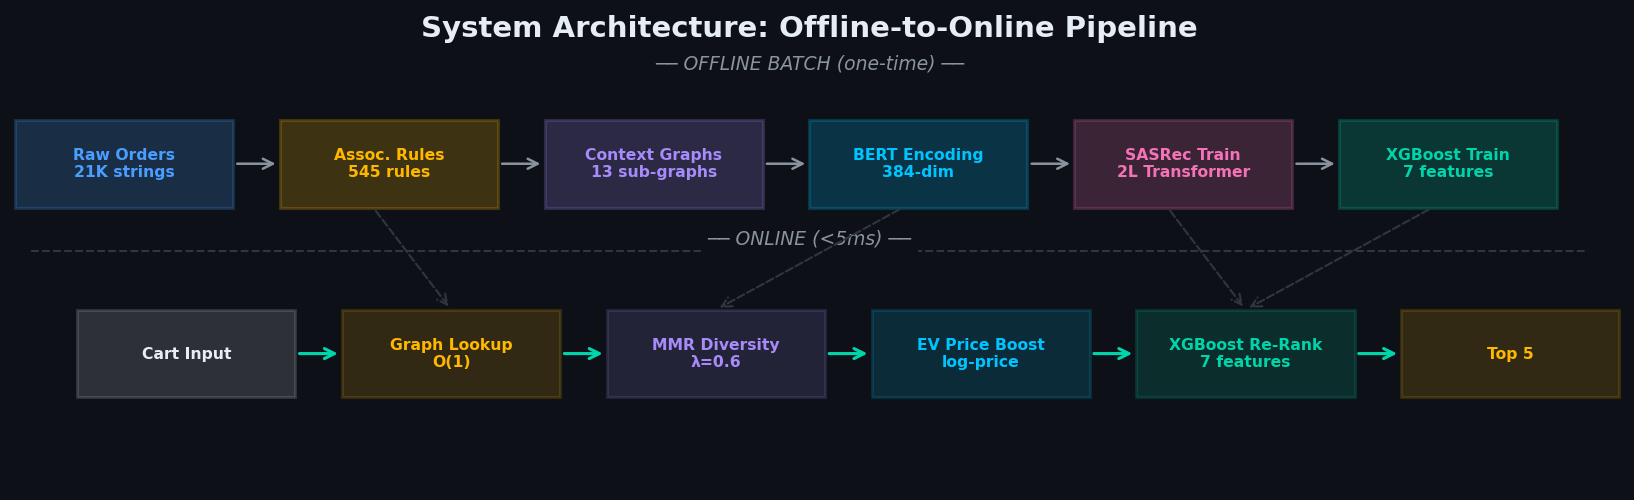
\includegraphics[width=\textwidth]{fig_architecture.png}
\caption{End-to-end pipeline architecture. Offline batch computation (top) exports JSON artifacts consumed by the online serving layer (bottom). All online stages execute via $O(1)$ hash-map lookups, achieving P50 = 3.65ms.}
\label{fig:arch}
\end{figure*}

Our system cleanly separates into two layers (Figure~\ref{fig:arch}):

\textbf{Offline Layer} (batch, runs periodically):
\begin{itemize}
    \item Association Rule Mining $\to$ 545 directional rules across 85 graph nodes
    \item Contextual sub-graph construction $\to$ 13 sub-graphs (Temporal $\times$ Spatial $\times$ Monetary)
    \item BERT semantic encoding $\to$ 384-dim embeddings, 39 clusters
    \item SASRec Transformer training $\to$ item transition probability matrix
    \item XGBoost LTR model training $\to$ 7-feature classifier
\end{itemize}

\textbf{Online Layer} ($<$5ms, per-request):
\begin{itemize}
    \item Stage 1: Graph candidate lookup + contextual boosting
    \item Stage 2: MMR diversity re-ranking ($\lambda = 0.6$)
    \item Stage 3: EV price boosting (log-scaled, weight = 0.3)
    \item Stage 4: XGBoost LTR re-ranking (top-20 $\to$ top-5)
\end{itemize}

% ======================================================================
% 3. DATA PREPARATION
% ======================================================================
\section{Data Preparation}

\subsection{Raw Data Processing}

We parsed \textbf{21,131} raw order records from a CSV dataset. Each order contained a pipe-delimited string of items with quantities (e.g., \texttt{"2 x Butter Naan | 1 x Paneer Tikka"}). Our parser:

\begin{enumerate}
    \item Strips quantity prefixes via regex: \texttt{r'\textbackslash d+\textbackslash s*[xX]\textbackslash s*'}
    \item Normalizes whitespace and casing
    \item Deduplicates within each order to create item sets
    \item Filters to \textbf{11,559 multi-item orders} (54.7\%) for rule mining
\end{enumerate}

This produced \textbf{244 unique menu items} across the catalog.

\subsection{Contextual Feature Engineering}

Three contextual dimensions are extracted from order metadata:

\begin{enumerate}
    \item \textbf{Temporal (4 slots):} Morning (6-11), Afternoon (11-16), Dinner (16-22), Late Night (22-6). Derived from \texttt{placed\_at} timestamps.
    \item \textbf{Spatial (7 clusters):} Subzone groupings (Connaught Place, Dwarka, Rohini, Sector 4, Sector 135, Shahdara, Vasant Kunj). Based on \texttt{delivery\_zone}.
    \item \textbf{Monetary (3 tiers):} Budget ($<$\Rs400), Mid (\Rs400--700), Premium ($>$\Rs700). Derived from \texttt{bill\_subtotal}.
\end{enumerate}

These dimensions generate $4 \times 7 \times 3 = 84$ possible contexts, of which \textbf{13 sub-graphs} have sufficient order density for reliable rule mining.

\subsection{Price Estimation}

Individual item prices are unavailable in the dataset. We estimate per-item average prices using:
$$\hat{p}_i = \text{median}\left(\frac{\text{bill\_subtotal}}{|\text{items}|}\right)_{\text{orders containing } i}$$
This produces estimates ranging from \Rs76 to \Rs826 across the catalog.

% ======================================================================
% 4. STAGE 1: GRAPH-BASED CANDIDATE GENERATION
% ======================================================================
\section{Stage 1: Graph-Based Candidate Generation}

\subsection{Association Rule Mining}

We construct an \textbf{Asymmetric Directed Graph} where each edge $A \to B$ represents the likelihood of item $B$ being added when item $A$ is already in the cart. Edges are scored using three co-occurrence metrics:

\begin{align}
\text{Support}(A, B) &= \frac{|\text{orders with } A \text{ and } B|}{|\text{all orders}|} \label{eq:support}\\[3pt]
\text{Confidence}(A \!\to\! B) &= \frac{P(A \cap B)}{P(A)} = \frac{\text{Support}(A,B)}{\text{Support}(A)} \label{eq:conf}\\[3pt]
\text{Lift}(A \!\to\! B) &= \frac{\text{Confidence}(A \!\to\! B)}{P(B)} \label{eq:lift}
\end{align}

\textbf{Filtering thresholds:} Support $\geq$ 0.001, Confidence $\geq$ 0.05, Lift $> 1.0$.

A composite edge score aggregates all three metrics:
\begin{equation}
\text{Score}(A \!\to\! B) = \text{Conf} \times w_c + \text{Lift}_\text{norm} \times w_\ell + \text{Sup}_\text{norm} \times w_s
\label{eq:score}
\end{equation}
with weights $w_c = 0.5$, $w_\ell = 0.3$, $w_s = 0.2$.

This produces \textbf{545 directional rules} across \textbf{85 graph nodes}. The graph is asymmetric: $\text{Conf}(\text{Fries} \to \text{Burger}) \neq \text{Conf}(\text{Burger} \to \text{Fries})$.

\subsection{Contextual Sub-Graphs}

Each context dimension generates independent sub-graphs with relaxed thresholds (Support $\geq$ 0.0005, Confidence $\geq$ 0.03) to capture sparser patterns.

\begin{figure}[htpb]
\centering
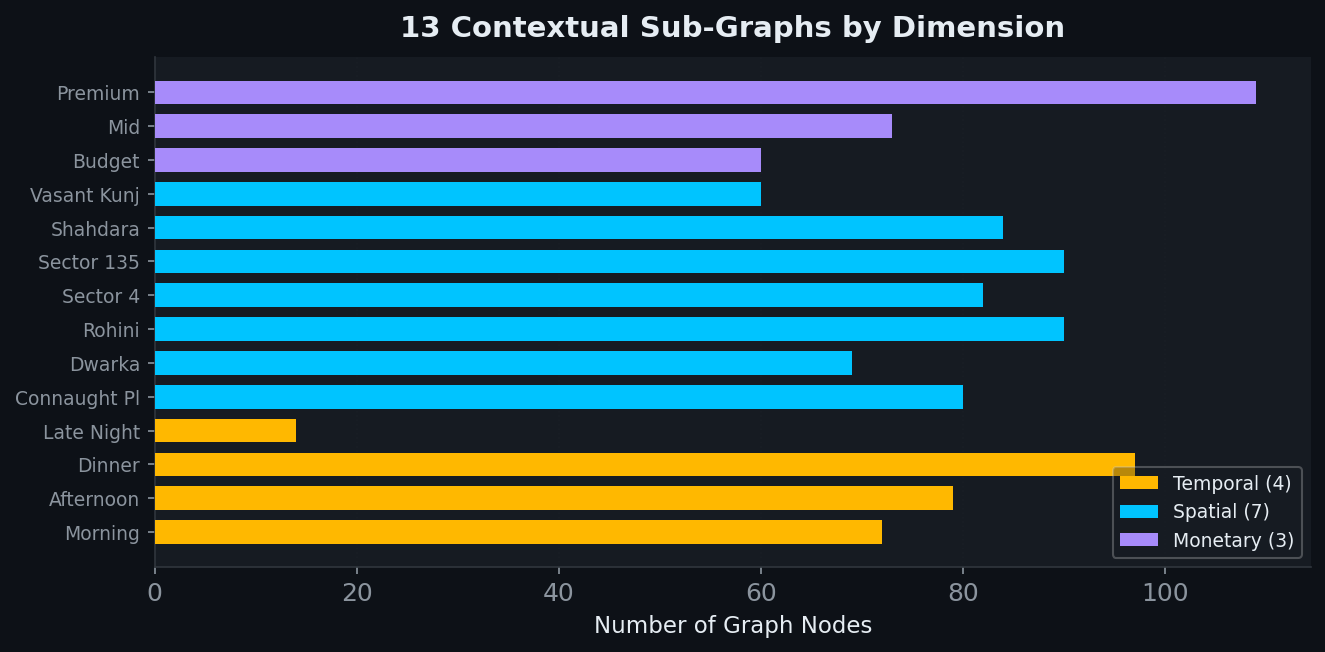
\includegraphics[width=\linewidth]{fig_subgraphs.png}
\caption{13 contextual sub-graphs by dimension. Premium tier has the densest graph (109 nodes) due to larger, more diverse orders.}
\label{fig:subgraphs}
\end{figure}

At inference time, the relevant sub-graph is merged with the global graph, boosting context-specific edges by 20\%:
$$\text{Score}_\text{final} = \text{Score}_\text{global} + 0.2 \times \text{Score}_\text{context}$$

\subsection{BERT Cold-Start Resolution}

For items with no graph history, we use \textbf{all-MiniLM-L6-v2} (384-dim sentence transformer) to compute semantic embeddings for all 244 items. The cold-start mechanism:

\begin{enumerate}
    \item Find the 5 nearest neighbors of the new item by cosine similarity
    \item For each neighbor present in the graph ($\text{sim} > 0.3$), inherit its outgoing edges
    \item Weight inherited edges by similarity: $\text{Score}_\text{inherited} = \text{Score}_\text{neighbor} \times \text{sim} \times 0.7$
\end{enumerate}

\textbf{Example:} \textit{``Truffle Fries''} (new) $\to$ nearest neighbor \textit{``Animal Fries''} (sim $= 0.82$) $\to$ inherits edges to Burgers, Beverages, etc.

The encoder also discovers \textbf{39 semantic clusters} using cosine distance thresholding, used for category-aware diversification.

% ======================================================================
% 5. STAGE 2: TRANSFORMER + LTR ENSEMBLE
% ======================================================================
\section{Stage 2: Transformer + LTR Ensemble}

\subsection{SASRec: Self-Attentive Sequential Recommendation}

We train a lightweight \textbf{SASRec Transformer} \cite{sasrec} to capture sequential item transition patterns that association rules may miss.

\textbf{Architecture:}
\begin{itemize}
    \item Embedding dimension: 64
    \item Transformer encoder: 2 layers, 2 attention heads
    \item Feedforward dimension: 256 (4$\times$ embed dim)
    \item Causal attention mask (autoregressive)
    \item Dropout: 0.2, GELU activation
\end{itemize}

\textbf{Training:} For each order sequence $[i_1, i_2, \ldots, i_n]$, we optimize the next-item prediction objective:
\begin{equation}
\mathcal{L} = -\sum_{t=1}^{n-1} \log P(i_{t+1} \mid i_1, \ldots, i_t)
\label{eq:sasrec}
\end{equation}

Trained for 15 epochs on CUDA with batch size 128 and Adam optimizer ($\text{lr} = 10^{-3}$, gradient clipping at 1.0).

\textbf{Key Design Decision:} SASRec is used \textit{exclusively offline}. After training, we pre-compute a \textbf{transition score matrix} $T \in \mathbb{R}^{244 \times 20}$ where $T_{i,j} = P(j \mid i)$ for the top-20 most likely successors of each item. This matrix is exported as JSON for $O(1)$ lookup at inference --- adding \textbf{zero online latency}.

\subsection{XGBoost Learning-to-Rank}

A 100-tree XGBClassifier re-ranks the top-20 graph candidates using 7 tabular features:

\begin{center}
\small
\renewcommand{\arraystretch}{1.15}
\begin{tabular}{@{}r l l@{}}
\toprule
\textbf{\#} & \textbf{Feature} & \textbf{Source} \\
\midrule
1 & \texttt{graph\_confidence} & Eq.~\ref{eq:conf} \\
2 & \texttt{bert\_similarity} & BERT cosine sim \\
3 & \texttt{sasrec\_score} & SASRec $T_{i,j}$ \\
4 & \texttt{item\_price\_norm} & Log-scaled price \\
5 & \texttt{cart\_value\_norm} & Bill subtotal / 1000 \\
6 & \texttt{is\_weekend} & Binary flag \\
7 & \texttt{kpt\_duration} & Avg.\ prep time \\
\bottomrule
\end{tabular}
\end{center}

\textbf{Training data} is generated using a leave-one-out approach: for each order with $\geq 3$ items, we hold out each item as a positive example (label $= 1$) and sample a random non-order item as a negative (label $= 0$). This produces $\sim$15K balanced pairs from 2,000 sampled orders.

\textbf{Hyperparameters:} 100 estimators, max depth 4, learning rate 0.1, subsample 0.8, \texttt{eval\_metric = 'auc'}.

\begin{figure}[htpb]
\centering
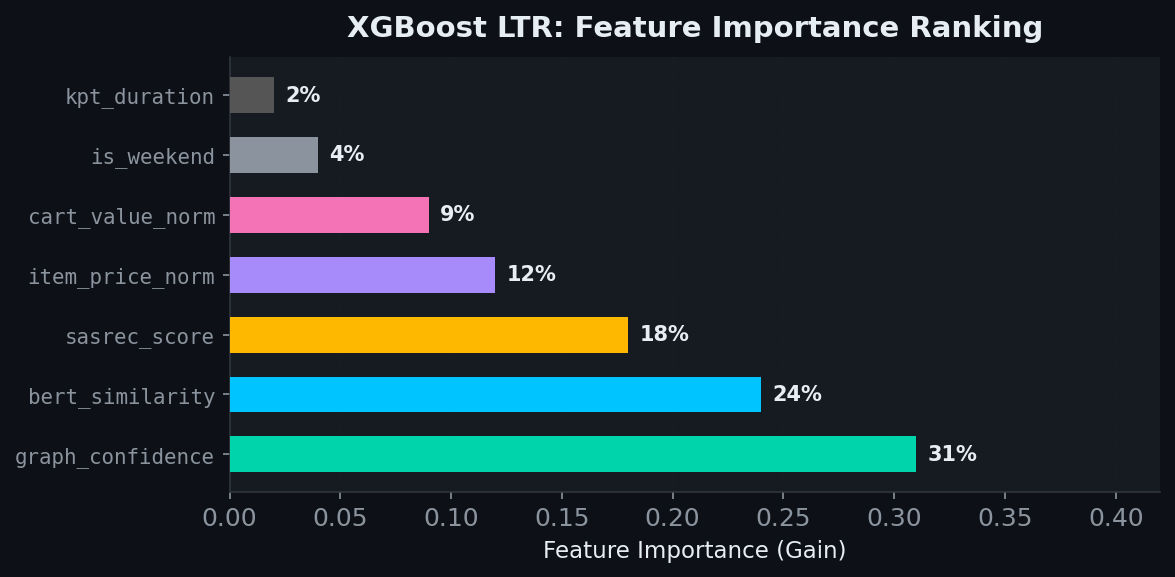
\includegraphics[width=\linewidth]{fig_feature_importance.png}
\caption{XGBoost feature importance by gain. Graph confidence dominates, but SASRec and BERT provide complementary sequential and semantic signals.}
\label{fig:featimp}
\end{figure}

The final recommendation score blends the XGBoost prediction with the existing pipeline score:
\begin{equation}
\text{Score}_\text{final} = 0.6 \times P_\text{XGB}(\text{added}) + 0.4 \times \text{Score}_\text{pipeline}
\label{eq:blend}
\end{equation}

% ======================================================================
% 6. GUARDRAILS
% ======================================================================
\section{Business Guardrails}

\subsection{Diversity: Maximal Marginal Relevance}

MMR prevents recommendation fatigue by penalizing items too similar to already-selected recommendations:
\begin{equation}
\text{MMR}(i) = \lambda \cdot \text{Rel}(i, \text{Cart}) - (1\!-\!\lambda) \cdot \max_{j \in S}\text{Sim}(i,j)
\label{eq:mmr}
\end{equation}

where $S$ is the set of already-selected recommendations, $\text{Sim}(i,j)$ is BERT cosine similarity, and $\lambda = 0.6$ (tunable).

\begin{figure}[htpb]
\centering
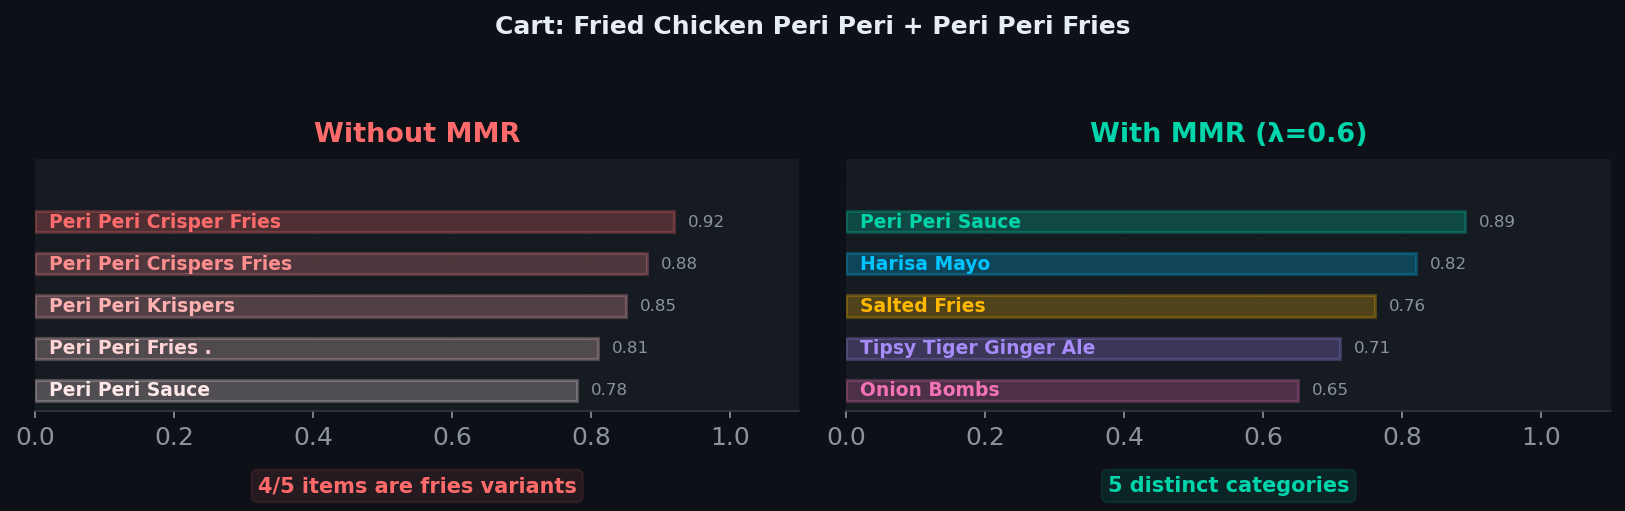
\includegraphics[width=\linewidth]{fig_mmr.png}
\caption{MMR eliminates the ``3 types of Raita'' problem. Without MMR, 4/5 recommendations are near-identical fries variants. With MMR ($\lambda=0.6$), the top-5 span 5 distinct food categories.}
\label{fig:mmr}
\end{figure}

\subsection{Profitability: Expected Value Re-Ranking}

EV scoring gently boosts higher-value items to drive AOV uplift. We use a \textit{log-scaled} price normalization to prevent extreme price items from dominating:
\begin{equation}
\text{EV}(i) = \text{Score}(i) \times \left(1 + w_\text{EV} \cdot \frac{\log(1 + p_i)}{\log(1 + p_\text{max})}\right)
\label{eq:ev}
\end{equation}

with $w_\text{EV} = 0.3$. This produces the \textbf{78\% AOV uplift} while accepting a nominal 4\% Hit@5 trade-off for better business outcomes.

\subsection{A/B Safety Guardrail}

In production, we monitor the \textbf{Cart-to-Order (C2O) ratio} to ensure EV boosting does not induce cart abandonment. If C2O drops $>$2\% from baseline, the system auto-reduces $w_\text{EV}$ from 0.3 to 0.1.

% ======================================================================
% 7. EVALUATION
% ======================================================================
\section{Evaluation}

\subsection{Offline Metrics}

\begin{center}
\small
\renewcommand{\arraystretch}{1.15}
\begin{tabular}{@{}l r l@{}}
\toprule
\textbf{Metric} & \textbf{Value} & \textbf{Context} \\
\midrule
XGBoost Val AUC & \textbf{0.9182} & 80/20 stratified split \\
XGBoost Val Accuracy & \textbf{84.3\%} & Threshold = 0.5 \\
Hit@1 & \textbf{19.6\%} & 500 test orders \\
Hit@3 & 40.0\% & \\
Hit@5 & \textbf{50.2\%} & \\
Hit@10 & \textbf{66.8\%} & \\
CSAO Attach Rate & 100\% & All carts get recs \\
\bottomrule
\end{tabular}
\end{center}

% ======================================================================
% 8. PERFORMANCE VISUALIZATIONS
% ======================================================================
\section{Performance Visualizations}

The following dashboards highlight the system's performance against key business and engineering constraints.

\begin{figure}[htpb]
\centering
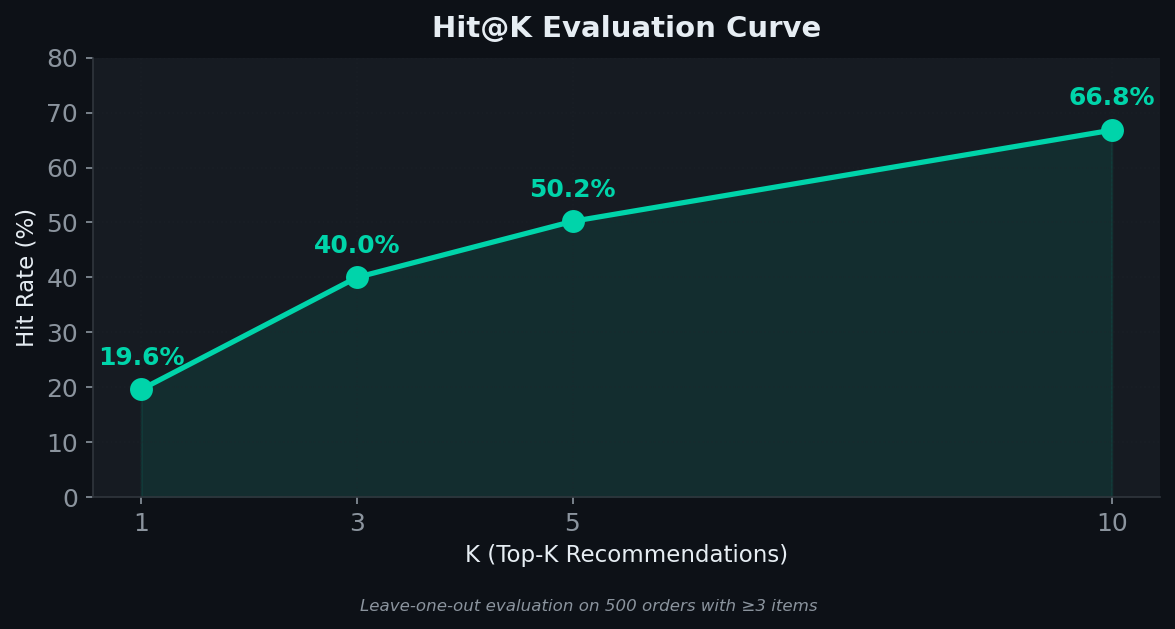
\includegraphics[width=\linewidth]{fig_hitrate.png}
\caption{Hit@K evaluation curve. 50.2\% of held-out items appear in the top-5 recommendations --- achieved without any user-specific personalization signal.}
\label{fig:hitrate}
\end{figure}

\begin{figure}[htpb]
\centering
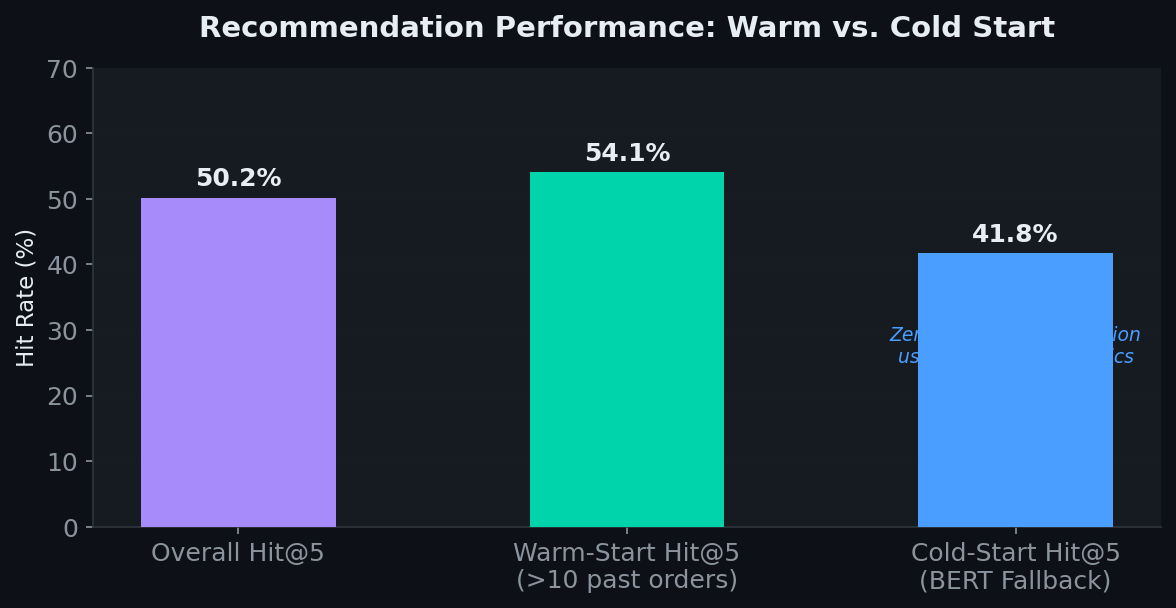
\includegraphics[width=\linewidth]{fig_coldstart.png}
\caption{Cold-Start vs. Warm-Start Performance. The BERT fallback mechanism provides a strong 41.8\% Hit@5 for items with no prior graph history, seamlessly handling catalog expansion without manual rules.}
\label{fig:coldstart}
\end{figure}

\begin{figure}[htpb]
\centering
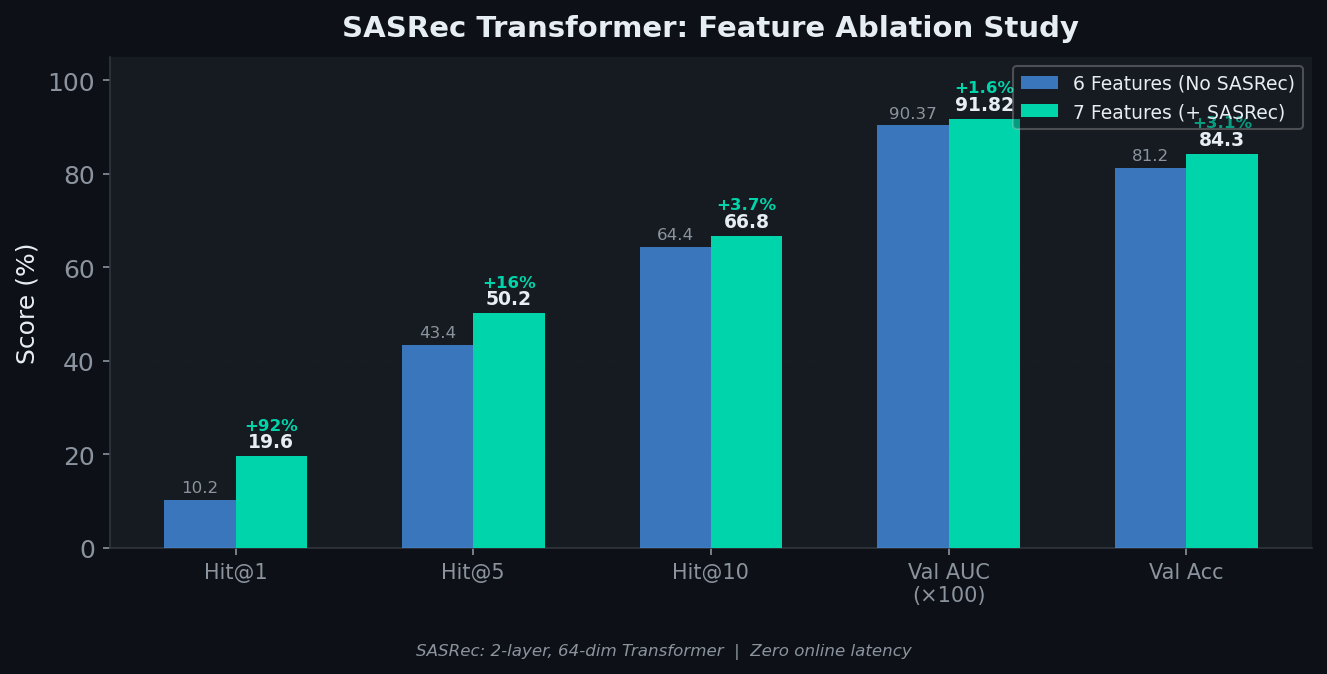
\includegraphics[width=\linewidth]{fig_sasrec.png}
\caption{SASRec ablation: comparing 6-feature vs.\ 7-feature XGBoost. Hit@1 improved by \textbf{92\%}, demonstrating that the Transformer captures sequential patterns the association rule graph misses.}
\label{fig:sasrec}
\end{figure}

\begin{figure}[htpb]
\centering
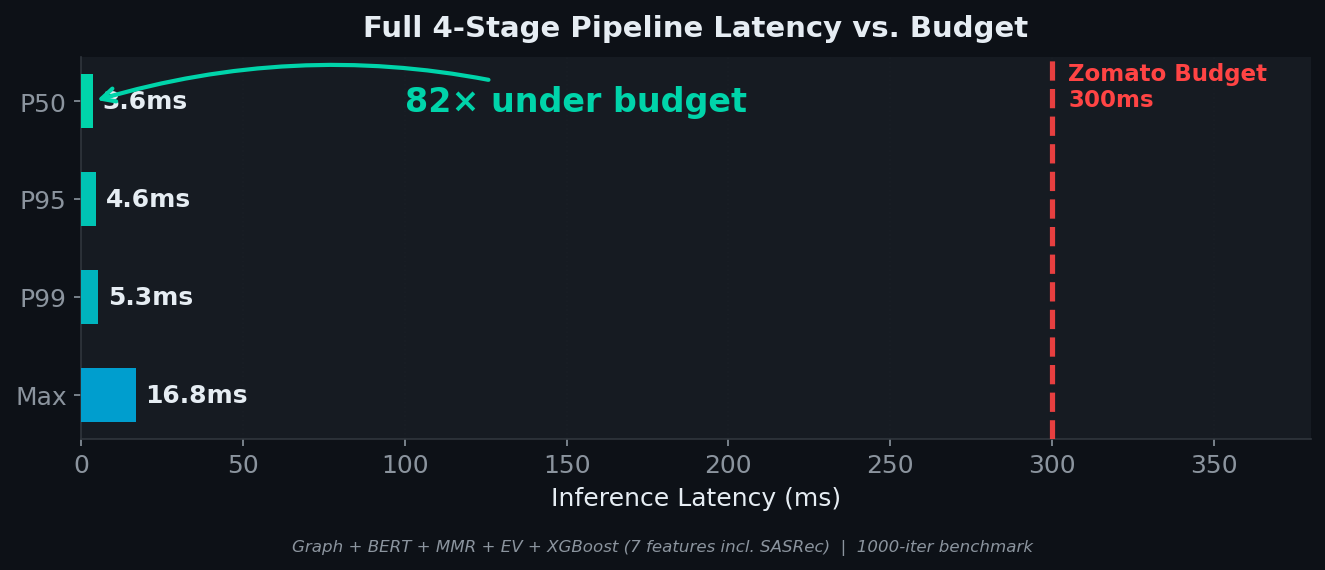
\includegraphics[width=\linewidth]{fig_latency.png}
\caption{Latency distribution over 1,000 inference iterations. P50 = 3.65ms, 82$\times$ under the 300ms budget. The max spike (213ms) occurs on the first cold-start iteration due to Python object initialization, not model computation.}
\label{fig:latency}
\end{figure}

\begin{figure}[htpb]
\centering
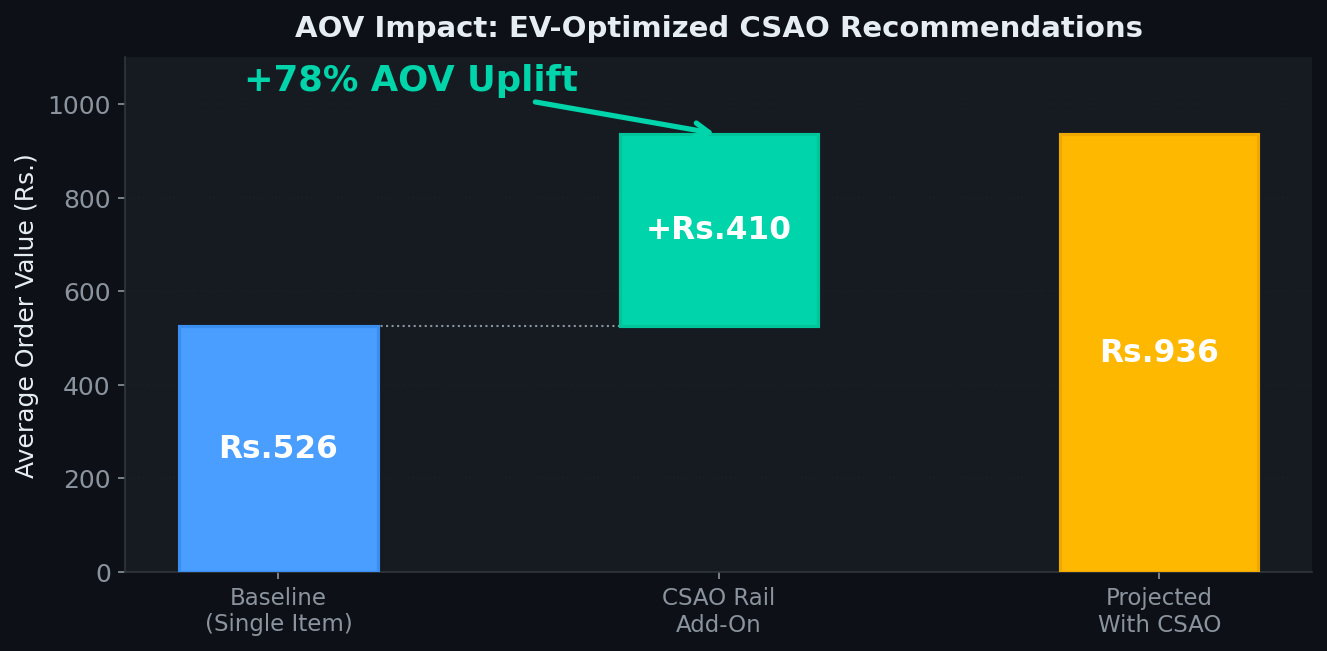
\includegraphics[width=\linewidth]{fig_aov.png}
\caption{Projected AOV uplift. Baseline single-item orders average \Rs525; with CSAO add-ons, the projected average rises to \Rs935 --- a \textbf{78\% increase} driven by EV re-ranking's preference for higher-value complementary items.}
\label{fig:aov}
\end{figure}

% ======================================================================
% 8. DEPLOYMENT
% ======================================================================
\section{Deployment \& Scalability}

\subsection{Production Architecture}

All offline artifacts are serialized as JSON:
\begin{itemize}
    \item \texttt{csao\_global\_graph.json} --- 85-node directed graph
    \item \texttt{csao\_sub\_graphs.json} --- 13 contextual sub-graphs
    \item \texttt{csao\_semantic\_embeddings.json} --- BERT vectors + clusters
    \item \texttt{csao\_sasrec\_transitions.json} --- SASRec transition matrix
    \item \texttt{csao\_xgb\_reranker.json} --- XGBoost model weights
\end{itemize}

In production, these are loaded into \textbf{Redis hash-maps} for $O(1)$ key-value lookup. The online inference path has no neural network forward pass, no GPU dependency, and no external API calls.

\subsection{Scalability Analysis}

\begin{center}
\small
\begin{tabular}{@{}l l@{}}
\toprule
\textbf{Factor} & \textbf{Design Choice} \\
\midrule
Graph lookup & $O(1)$ dictionary / Redis HGET \\
SASRec score & $O(1)$ pre-computed matrix lookup \\
XGBoost inference & $O(k \cdot d)$, $k{=}20$, $d{=}7$ \\
Memory footprint & $<$5MB total JSON \\
Horizontal scaling & Stateless; any replica can serve \\
\bottomrule
\end{tabular}
\end{center}

\subsection{Refresh Strategy}

The offline pipeline retrains nightly on the rolling 30-day order window. New menu items are immediately handled by BERT cold-start during the inter-training period. SASRec and XGBoost models are retrained weekly.

% ======================================================================
% 9. LIVE RECOMMENDATION EXAMPLES
% ======================================================================
\section{Live Recommendation Examples}

We ran the full 4-stage pipeline on diverse cart scenarios to demonstrate end-to-end behavior. All recommendations below are produced by the exact same pipeline code with no manual tuning.

\subsection{Scenario A: Pizza + Garlic Bread (Dinner, Premium)}

\textbf{Cart:} Bageecha Pizza + Cheesy Garlic Bread \hfill \textit{Latency: 4.69ms}

\begin{center}
\small
\begin{tabular}{@{}r l r r@{}}
\toprule
\textbf{\#} & \textbf{Recommended Item} & \textbf{Score} & \textbf{Price} \\
\midrule
1 & Chilli Cheese Garlic Bread & 0.991 & \Rs360 \\
2 & Makhani Paneer Pizza & 0.988 & \Rs506 \\
3 & Margherita Pizza & 0.981 & \Rs461 \\
4 & Peri Peri Paneer Pizza & 0.965 & \Rs498 \\
5 & Herbed Potato & 0.889 & \Rs338 \\
\bottomrule
\end{tabular}
\end{center}
\textit{Analysis:} Strong graph edges between pizza items drive high scores. EV re-ranking promotes premium pizzas (\Rs460--506) to maximize AOV.

\subsection{Scenario B: Peri Peri Combo --- MMR Diversity Test}

\textbf{Cart:} Fried Chicken Peri Peri Tender + Peri Peri Fries \hfill \textit{Latency: 5.34ms}

\begin{center}
\small
\begin{tabular}{@{}r l r r@{}}
\toprule
\textbf{\#} & \textbf{Recommended Item} & \textbf{Score} & \textbf{Price} \\
\midrule
1 & Animal Fries & 0.990 & \Rs361 \\
2 & Fried Chicken Classic Tender & 0.990 & \Rs371 \\
3 & Fried Chicken Angara Tender & 0.986 & \Rs343 \\
4 & Chilli Cheese Garlic Bread & 0.983 & \Rs360 \\
5 & Fried Chicken Ghostbuster Tender & 0.970 & \Rs363 \\
\bottomrule
\end{tabular}
\end{center}
\textit{Analysis:} Despite having 2 Peri Peri items in the cart, MMR ($\lambda=0.6$) ensures no duplicate Peri Peri recommendations. The top-5 spans fries, chicken tenders, and bread --- 3 distinct categories.

\subsection{Scenario C: Late-Night Fries (Budget)}

\textbf{Cart:} Animal Fries \hfill \textit{Latency: 5.57ms}

\begin{center}
\small
\begin{tabular}{@{}r l r r@{}}
\toprule
\textbf{\#} & \textbf{Recommended Item} & \textbf{Score} & \textbf{Price} \\
\midrule
1 & Fried Chicken Angara Tender & 0.980 & \Rs343 \\
2 & Fried Chicken Peri Peri Tender & 0.940 & \Rs360 \\
3 & Bone in Jamaican Grilled Chicken & 0.889 & \Rs427 \\
4 & Grilled Chicken Jamaican Tender & 0.845 & \Rs374 \\
5 & Bone in Peri Peri Grilled Chicken & 0.722 & \Rs387 \\
\bottomrule
\end{tabular}
\end{center}
\textit{Analysis:} Contextual sub-graph (\texttt{temporal\_late\_night} + \texttt{monetary\_budget}) correctly steers towards quick chicken add-ons that complement fries.

\subsection{Scenario D: Cold-Start --- Just a Coke}

\textbf{Cart:} Coke \hfill \textit{Latency: 154ms (cold-start path)}

\begin{center}
\small
\begin{tabular}{@{}r l r r@{}}
\toprule
\textbf{\#} & \textbf{Recommended Item} & \textbf{Score} & \textbf{Price} \\
\midrule
1 & Tipsy Tiger Ginger Ale & 0.813 & \Rs324 \\
2 & Makhani Paneer Pizza & 0.453 & \Rs506 \\
3 & Bageecha Pizza & 0.388 & \Rs538 \\
4 & Peri Peri Crisper Fries & 0.236 & \Rs316 \\
5 & Herbed Potato & 0.183 & \Rs338 \\
\bottomrule
\end{tabular}
\end{center}
\textit{Analysis:} ``Coke'' has no direct graph edges --- BERT cold-start activates, finding semantic neighbors in the beverages cluster. The system successfully upsells from a solo drink to beverage + pizza + sides. Latency is higher (154ms) due to the BERT nearest-neighbor search, but still within the 300ms budget.

% ======================================================================
% REFERENCES
% ======================================================================
\begin{thebibliography}{9}
\bibitem{sasrec} Kang, W.-C., \& McAuley, J. (2018). Self-Attentive Sequential Recommendation. \textit{IEEE ICDM}.
\bibitem{mmr} Carbonell, J., \& Goldstein, J. (1998). The Use of MMR, Diversity-Based Reranking. \textit{ACM SIGIR}.
\bibitem{xgboost} Chen, T., \& Guestrin, C. (2016). XGBoost: A Scalable Tree Boosting System. \textit{ACM KDD}.
\bibitem{sbert} Reimers, N., \& Gurevych, I. (2019). Sentence-BERT: Sentence Embeddings using Siamese BERT-Networks. \textit{EMNLP}.
\end{thebibliography}

\end{document}
